
\documentclass{exam}

\usepackage{graphicx}
\usepackage[fleqn]{amsmath}
\usepackage{unitsdef} 
\usepackage{cancel}
\usepackage{float}
\usepackage{mdwlist}
\usepackage{booktabs}
\usepackage{cancel}
\usepackage{polynom}
\usepackage{caption}
\usepackage{fullpage}
\usepackage{enumerate}
% \usepackage{parskip}

% \newcommand{\degree}{\ensuremath{^\circ}} 
\everymath{\displaystyle}

\newunit{\inch}{in}
\newunit{\foot}{ft}
\newunit{\cemtimeter}{cm}

% \begin{figure}[H]
%   \centering
%   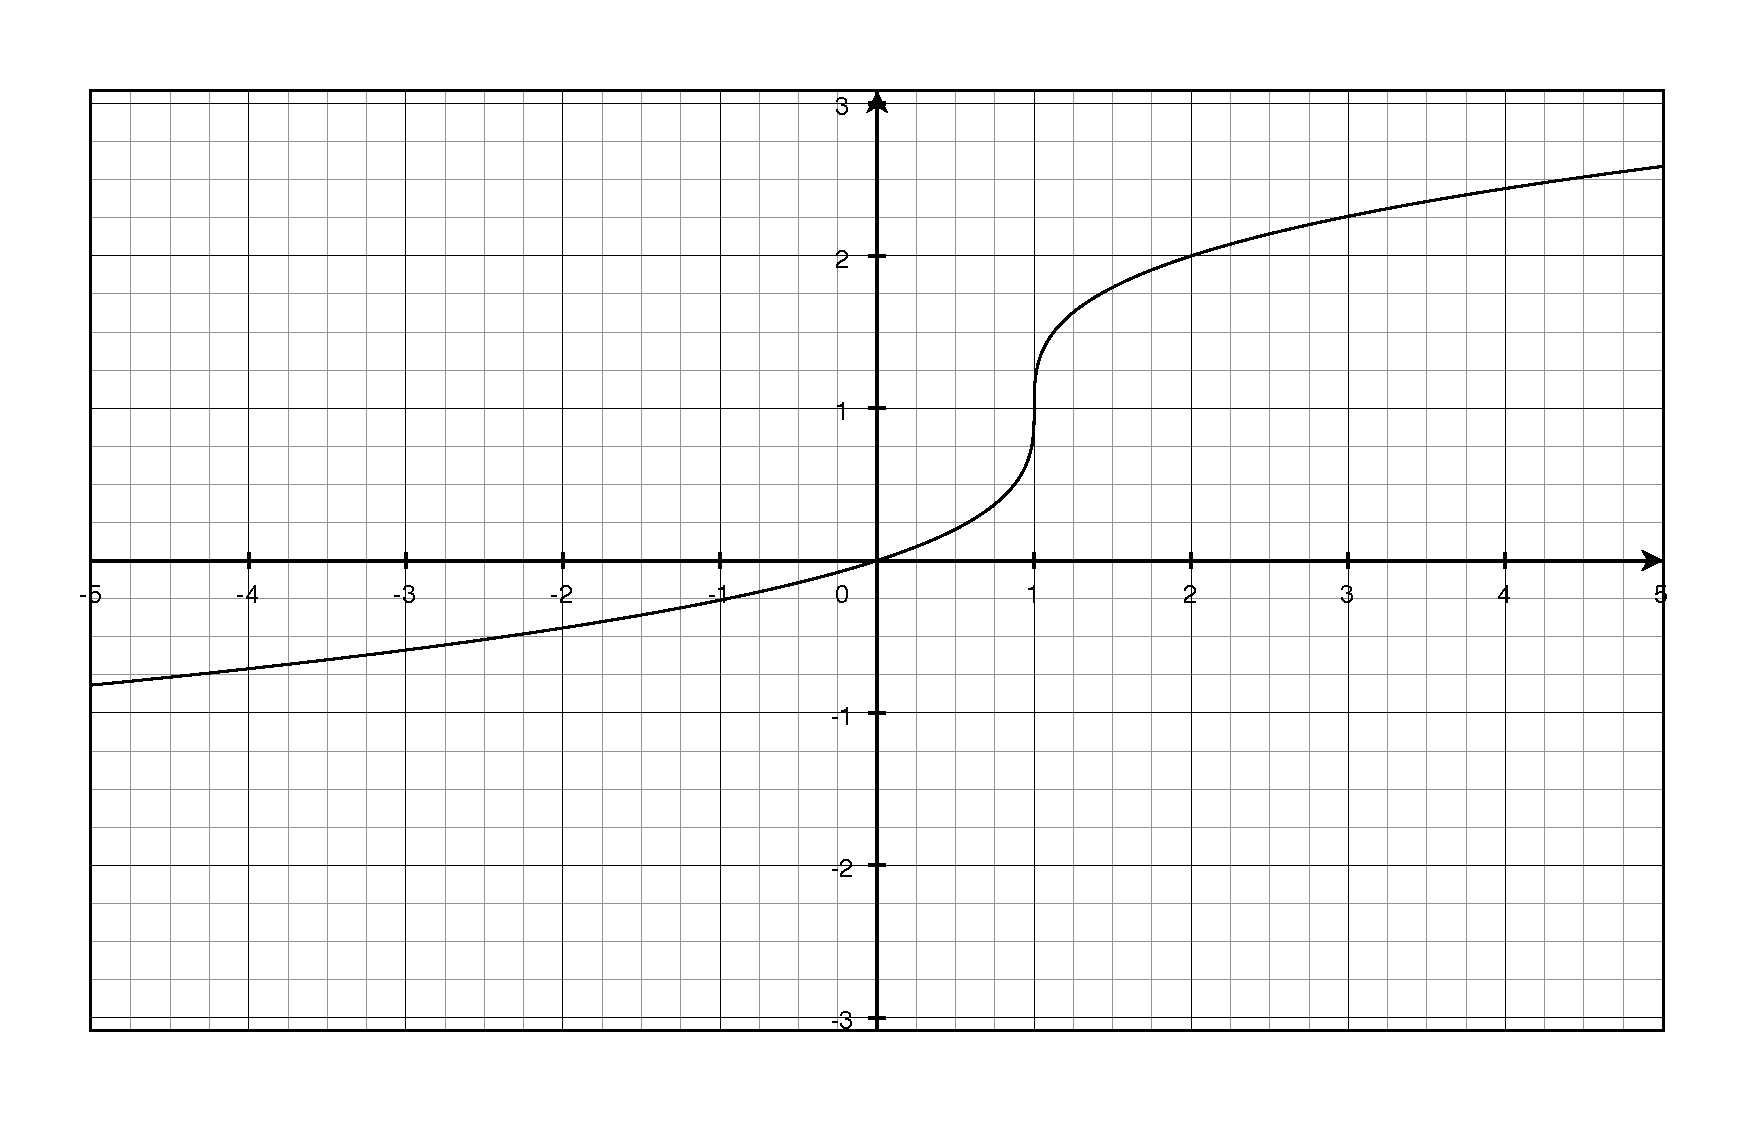
\includegraphics[scale=.3]{question7.eps}
%   \caption*{Question 7}
% \end{figure}

% \begin{tabular}{cc}
% \toprule
% period & amplitude \\
% \midrule
%   $\pi$ & $2$ \\
% \bottomrule
% \end{tabular}

\printanswers

\ifprintanswers 
\usepackage{2in1, lscape} 
\fi

\title{Math 263B \\ Homework Twelve}
\date{December 6, 2012}

\begin{document}

\maketitle

\section{Homework}

\begin{itemize*}
  \item Read Section 7.3
  \item pp 364-365: 1-18
\end{itemize*}

%% \ifprintanswers
%% \pagebreak
%% \fi

\section{Extra Credit}
page 364, problem 19
\ifprintanswers
\begin{solution}
The first thing to look at is the expression $\sqrt{x^2}$.  This is equivalent to $|x|$, since you end up with the
original value with the sign removed by the square/square root operations.  This means the original equation is
actually:
\begin{align*}
  y &= \sqrt{e^{x^2}} + e^{\sqrt{x^2}} \\
    &= \left( e^{x^2} \right)^{1/2} + e^{|x|} \\
    &= e^{x^2/2} + e^{|x|} \\
\end{align*}

We can write this as two different equations 
\[
  y = \begin{cases}
        e^{x^2/2} + e^{x}  & \text{if } x \geq 0 \\
        e^{x^2/2} + e^{-x} & \text{if } x < 0 \\
      \end{cases}
\]

So the derivative is:
\[
  y = \begin{cases}
        x e^{x^2/2} + e^{x}  & \text{if } x \geq 0 \\
        x e^{x^2/2} - e^{-x} & \text{if } x < 0 \\
      \end{cases}
\]
 
\end{solution}

\section{Section 7.3}

\begin{description}
\item[3]
\[
  e^{3 \ln x} = x^3
\]

\item[4]
\[
  e^{-2 \ln x} = \frac{1}{x^2}
\]

\item[5]
\[
  \ln e^{\cos x} = \cos x
\]

\item[6]
\[
  \ln e^{-2x - 3} = -2x - 3
\]

\item[7]
\[
  \ln (x^3 e^{-3x}) = \ln x^3 + \ln e^{-3x} = 3 \ln x - 3x
\]

\item[8]
\[
  e^{x - \ln x} = e^x \cdot e^{- \ln x} = \frac{e^x}{x}
\]

\item[9]
\[
  e^{\ln 3 + 2 \ln x} = e^{\ln 3} \cdot e^{2 \ln x} = 3x^2 
\]

\item[10]
\[
  e^{2 \ln x - y \ln x} = e^{\ln x(2 - y)} = x^{2 - y}
\]


\item[11]
\begin{align*}
  y  &= e^{x + 2} \\
  y' &= e^{x + 2} \\
\end{align*}

\item[12]
\begin{align*}
  y  &= e^{2x^2 - x} \\
  y  &= e^{2x^2 - x} \cdot (4x - 1) \\
\end{align*}

\item[13]
\begin{align*}
  y  &= e^{\sqrt{x + 2}} \\
  y' &= e^{\sqrt{x + 2}} \cdot \frac{1}{2} (x + 2)^{-1/2} \\
     &= \frac{e^{\sqrt{x + 2}} } {2 \sqrt{x + 2}} \\
\end{align*}

\item[14]
\begin{align*}
  y &= e^{-1/x^2} \\
    &= e^{-x^{-2}} \\
  y' &= e^{-x^{-2}} \cdot 2x^{-3} \\
     &= \frac{2 e^{-1/x^2}}{x^3} \\
\end{align*}

\item[15]
\begin{align*}
  y &= e^{2 \ln x} \\
    &= x^2 \\
  y' &= 2x \\
\end{align*}

\item[16]
\begin{align*}
  y &= e^{x/\ln x} \\
  y' &= e^{x/\ln x} \cdot D_x \frac{x}{\ln x} \\
     &= e^{x/\ln x} \cdot \frac{\ln x - 1}{(\ln x)^2} \\
\end{align*}

\item[17]
\begin{align*}
  y &= x^3 e^x \\
  y' &= x^3 e^x + 3x^2 e^x \\
     &= e^x (x^3 + 3x^2) \\
     &= x^2 e^x (x + 3) \\
\end{align*}

\item[18]
\begin{align*}
  y &= e^{x^3 \ln x} \\
  y' &= e^{x^3 \ln x} \cdot D_x x^3 \ln x \\
     &= e^{x^3 \ln x} \cdot (x^3 \cdot \frac{1}{x} + \ln x \cdot 3x^2) \\
     &= x^2 e^{x^3 \ln x} \cdot (1 + 3 \ln x) \\
\end{align*}


\end{description}

\else

\vspace{11 cm} {\em Value judgments are destructive to our proper business, which is curiosity and awareness.}

\hspace{0.5 cm} --John Cage

\fi

\end{document}

